直線とカーブ両方あり,周期境界条件を持ち複数の対面走行できるように,
楕円コースで実験する.
コースの中(青い部分)にロボットをランダムに配置し,半数のロボットが右回り
($b_{\rm L}>b_{\rm R}$),
残りのロボットが左回り($b_{\rm L}<b_{\rm R}$)の向きで,
速度0からほぼ同時にスタート,約8分間実験する.

ロボットがtof距離センサーでコースの障害物までの距離を測って,
非線形感覚運動写像モデルにより走行する.

コースの青い部分の中央(図\ref{fig:cource}黒い線)でコースの長さを測る,
コースの長さ($L$)は7.32$m$,今回ロボットの台数($N$)は8台.
ロボットの線密度 $ \rho = \frac{N}{L} = 1.09 ({\rm 台/m})$

両側の壁を移動させて,コースの幅($w$)を
$43cm$,$49.5cm$,$56cm$,$62.5cm$,$69cm$へ変化させ,実験する.

\begin{eqnarray}
Q_i &=& \frac{|n_i|}{wT_{\rm sd}}
\label{eq:flow} \\
\bar{Q} &=& \frac{1}{N_{\rm exp}}\sum_{i=1}^{N_{\rm exp}} Q_i
\label{eq:flow_ave} 
\end{eqnarray}

\begin{figure}[h]
    \begin{minipage}{0.48\linewidth}
        \centering
        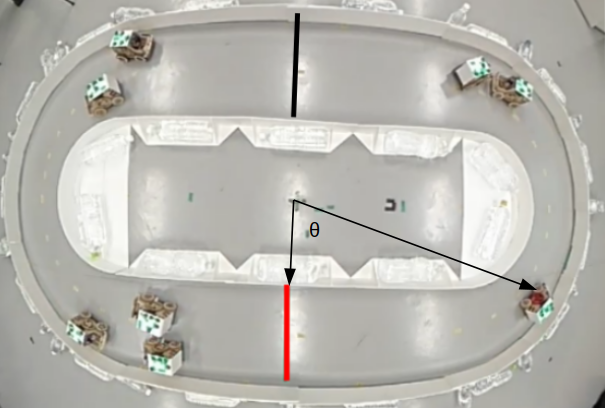
\includegraphics[width=0.9\linewidth]{course3.jpg}
        \caption{コース}
    \end{minipage}
    \begin{minipage}{0.48\linewidth}
        \centering
        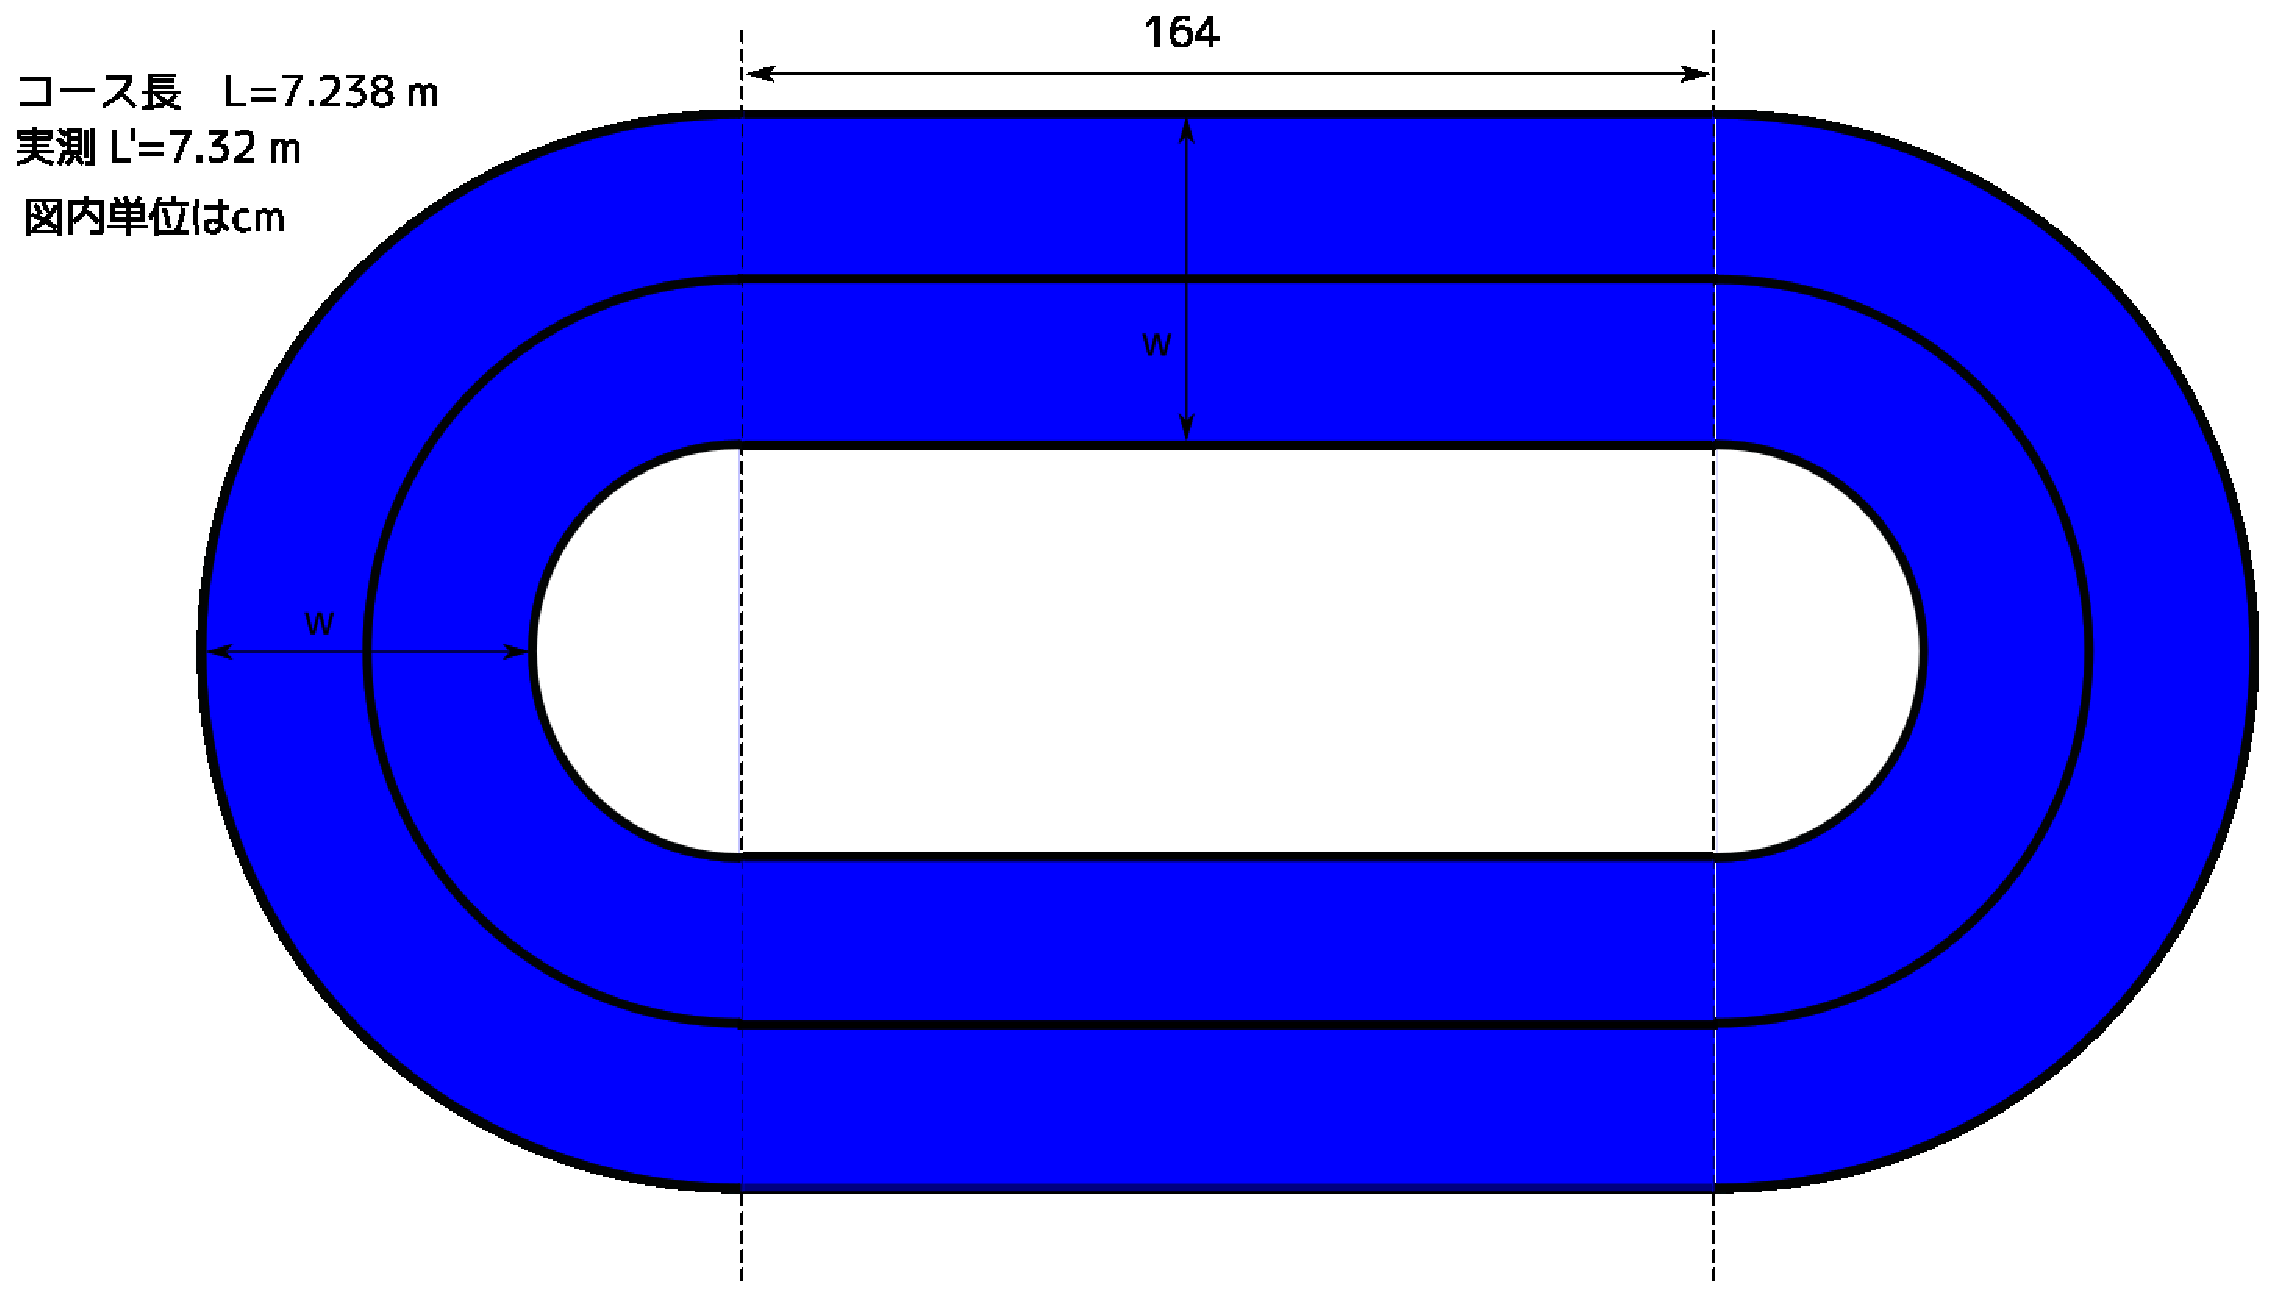
\includegraphics[width=1.0\linewidth]{Oval_h2.eps}
        \caption{\label{fig:cource}コースレイアウト}
    \end{minipage}
\end{figure}



図5の赤い線を計測ラインとして,ロボットが左から右へ線を通過したら流量+1,右から左へ線を通過したら流量-1.図6の横軸が時間(秒),縦軸がコース中心からみたロボットの位置角度$\theta$(図5),ロボットが赤い線から反時計回りで黒い線まで,$\theta$が0から$\pi$に変わる.赤い線から時計回りで黒い線まで,$\theta$が0から$-\pi$に変わる.横軸の時間に従う,$\theta$の変化が$0$を跨ぐと,計測ライン(赤い線)を通過したと認めて,台数($n$)を計測する.$T_{\rm sd}$はone direction flow 状態になる時間(分),$w$がコースの幅(単位:$m$),$Q$が流量,式6で流量を計算する.

